\documentclass[11pt]{amsart}

\usepackage{amsmath,amsthm}
\usepackage{amssymb}
\usepackage{graphicx}
\usepackage{enumerate}
\usepackage{fullpage}
% \usepackage{euscript}
% \makeatletter
% \nopagenumbers
\usepackage{verbatim}
\usepackage{color}
\usepackage{hyperref}
%\usepackage{times} %, mathtime}

\textheight=600pt %574pt
\textwidth=480pt %432pt
\topmargin=10pt %14.21pt

\parskip=1pt %2pt

% define theorem environments
\newtheorem{theorem}{Theorem}    %[section]
%\def\thetheorem{\unskip}
\newtheorem{proposition}[theorem]{Proposition}
%\def\theproposition{\unskip}
\newtheorem{conjecture}[theorem]{Conjecture}
\def\theconjecture{\unskip}
\newtheorem{corollary}[theorem]{Corollary}
\newtheorem{lemma}[theorem]{Lemma}
\newtheorem{sublemma}[theorem]{Sublemma}
\newtheorem{fact}[theorem]{Fact}
\newtheorem{observation}[theorem]{Observation}
%\def\thelemma{\unskip}
\theoremstyle{definition}
\newtheorem{definition}{Definition}
%\def\thedefinition{\unskip}
\newtheorem{notation}[definition]{Notation}
\newtheorem{remark}[definition]{Remark}
% \def\theremark{\unskip}
\newtheorem{question}[definition]{Question}
\newtheorem{questions}[definition]{Questions}
%\def\thequestion{\unskip}
\newtheorem{example}[definition]{Example}
%\def\theexample{\unskip}
\newtheorem{problem}[definition]{Problem}
\newtheorem{exercise}[definition]{Exercise}

\numberwithin{theorem}{section}
\numberwithin{definition}{section}
\numberwithin{equation}{section}

\def\reals{{\mathbb R}}
\def\torus{{\mathbb T}}
\def\integers{{\mathbb Z}}
\def\rationals{{\mathbb Q}}
\def\naturals{{\mathbb N}}
\def\complex{{\mathbb C}\/}
\def\distance{\operatorname{distance}\,}
\def\support{\operatorname{support}\,}
\def\dist{\operatorname{dist}\,}
\def\Span{\operatorname{span}\,}
\def\degree{\operatorname{degree}\,}
\def\kernel{\operatorname{kernel}\,}
\def\dim{\operatorname{dim}\,}
\def\codim{\operatorname{codim}}
\def\trace{\operatorname{trace\,}}
\def\dimension{\operatorname{dimension}\,}
\def\codimension{\operatorname{codimension}\,}
\def\nullspace{\scriptk}
\def\kernel{\operatorname{Ker}}
\def\p{\partial}
\def\Re{\operatorname{Re\,} }
\def\Im{\operatorname{Im\,} }
\def\ov{\overline}
\def\eps{\varepsilon}
\def\lt{L^2}
\def\curl{\operatorname{curl}}
\def\divergence{\operatorname{div}}
\newcommand{\norm}[1]{ \|  #1 \|}
\def\expect{\mathbb E}
\def\bull{$\bullet$\ }
\def\det{\operatorname{det}}
\def\Det{\operatorname{Det}}
\def\rank{\mathbf r}
\def\diameter{\operatorname{diameter}}

\def\t2{\tfrac12}

\newcommand{\abr}[1]{ \langle  #1 \rangle}

\def\newbull{\medskip\noindent $\bullet$\ }
\def\field{{\mathbb F}}
\def\cc{C_c}



% \renewcommand\forall{\ \forall\,}

% \newcommand{\Norm}[1]{ \left\|  #1 \right\| }
\newcommand{\Norm}[1]{ \Big\|  #1 \Big\| }
\newcommand{\set}[1]{ \left\{ #1 \right\} }
%\newcommand{\ifof}{\Leftrightarrow}
\def\one{{\mathbf 1}}
\newcommand{\modulo}[2]{[#1]_{#2}}

\def\bd{\operatorname{bd}\,}
\def\cl{\text{cl}}
\def\nobull{\noindent$\bullet$\ }

\def\scriptf{{\mathcal F}}
\def\scriptq{{\mathcal Q}}
\def\scriptg{{\mathcal G}}
\def\scriptm{{\mathcal M}}
\def\scriptb{{\mathcal B}}
\def\scriptc{{\mathcal C}}
\def\scriptt{{\mathcal T}}
\def\scripti{{\mathcal I}}
\def\scripte{{\mathcal E}}
\def\scriptv{{\mathcal V}}
\def\scriptw{{\mathcal W}}
\def\scriptu{{\mathcal U}}
\def\scriptS{{\mathcal S}}
\def\scripta{{\mathcal A}}
\def\scriptr{{\mathcal R}}
\def\scripto{{\mathcal O}}
\def\scripth{{\mathcal H}}
\def\scriptd{{\mathcal D}}
\def\scriptl{{\mathcal L}}
\def\scriptn{{\mathcal N}}
\def\scriptp{{\mathcal P}}
\def\scriptk{{\mathcal K}}
\def\scriptP{{\mathcal P}}
\def\scriptj{{\mathcal J}}
\def\scriptz{{\mathcal Z}}
\def\scripts{{\mathcal S}}
\def\scriptx{{\mathcal X}}
\def\scripty{{\mathcal Y}}
\def\frakv{{\mathfrak V}}
\def\frakG{{\mathfrak G}}
\def\aff{\operatorname{Aff}}
\def\frakB{{\mathfrak B}}
\def\frakC{{\mathfrak C}}

\def\suchthat{\mathrel{}:\mathrel{}}
\def\symdif{\,\Delta\,}
\def\mustar{\mu^*}
\def\muplus{\mu^+}

\def\soln{\noindent {\bf Solution.}\ }


%\pagestyle{empty}
%\setlength{\parindent}{0pt}

\begin{document}

\begin{center}{\bf Math 202A --- UCB, Fall 2016 --- William Guss}
\\
{\bf Problem Set 8, due Wednesday October 19}
\end{center}

\medskip \noindent {\bf (8.1)}\ (Folland problem 3.9)\ 
Let $\nu_j$ be a sequence of positive measures on a measurable space $(X,\scriptm)$,
and let $\mu$ be a positive measure on $(X,\scriptm)$.
Set $\nu = \sum_j \nu_j$.
Show that if $\nu_j\perp \mu$ for all $j$ then $\nu\perp\mu$,
and that if $\nu_j\ll \mu$ for all $j$ then $\nu\ll\mu$.

\begin{proof}
	We first show that if $\nu \perp \mu$ for all $j$ then $\nu \perp \mu$.
	For every $j$ $\nu_ \perp \mu$ if and only if there exist $A_j, B_j$ so that
	$\nu_(A_j) = 0$ and $\mu(B_j) = 0$. Then since $B_j$ is a countable collection of  $\mu$-null sets
	$\mu(\bigcup B_j) = 0$. Now $X \setminus \bigcup B_j = \bigcap A_j = A$ (follows from $B_j^C = A_j$) has the property that 
	$\nu_j(A) = 0$ for all $j$; that is, $\nu(A) = \sum \nu(A) = 0$. Finally $A \cup \bigcup B_j = X$.

	We now show that if $\nu_j\ll \mu$ for all $j$ then $\nu\ll\mu$. Take $E \in \scriptm$
	so that $\mu(E) = 0$. Then $\nu(E) = 0$ for all $j$ and
	$\nu(E) = \sum \nu_j(E) = \sum 0 = 0$, and so if $\mu(E) = 0$ then $\nu(E) = 0$ and
	$\nu \ll \mu$.
\end{proof}

\medskip \noindent {\bf (8.2)}\ (Folland problem 3.11(b))\ 
Let $\mu$ be a positive measure on $(X,\scriptm)$.
A family of functions $\{f_\alpha: \alpha\in A\}\subset L^1(\mu)$
is said to be uniformly integrable if for every $\eps>0$
there exists $\delta>0$ such that $\mu(E)<\delta
\Rightarrow |\int_E f_\alpha\,d\mu|<\eps$ for every $\alpha\in A$.
Let $A=\naturals$.
Show that if $f\in L^1(\mu)$ and if $f_n\to f$ in the $L^1$ ``metric''
then $\{f_n: n\in\naturals\}$ is uniformly integrable.
\begin{proof}
	To prove the statement we will show that $|\int f_\alpha|$ is bounded by
	$|\int f|$ and $|\int f_n -f|$ and then reason that there exist small enough mutual domains to both integrals so that 
	the bound is as small as we like.

	Let $\epsilon > 0$ be given.
	First for any $E$ observe that because $f_n, f \in L^1(\mu)$ 
	\begin{equation*}
		\left|\int_E f_n d\mu\right| = \left|\int_E f_n -f + f d\mu\right| \leq \left|\int_E f_n -f d\mu\right| + \left|\int_E  \int f d\mu\right|
	\end{equation*}
	Since $f \in L^1(\mu)$ by Corollary 3.6 there is a $\delta > 0$ such that $|\int_E f\ d\mu| < \epsilon/2$ whenever $\mu(E) < \delta$. 

	Now it remains to show that $\{f_n -f\}$ is uniformly integrable. Since $f_n \to f$ in $L^1(\mu)$ there is an $N$ such that
	for all $m \geq N$ $\int_X |f_m - f| d\mu < \epsilon/2$. Because $f_m - f \in L^1(\mu)$
	\begin{equation*}
		\left|\int_E f_m -f d\mu\right| \leq\int_E \left| f_m - f\right| d\mu \leq\int_X \left| f_m  -f \right| d\mu < \epsilon/2,
	\end{equation*}
	and the famlily  $\{f_m -f\ :\ m \geq N\}$ is uniformly integrable. Now consider the finite family $F^* = \{f_m -f\ :\ n < N\}$. For every $\phi_n \in F^*$ there is a $\delta_n > 0$ so that $|\int_E \phi_n d\mu| < \epsilon/2$ as long as $\mu(E) < \delta_n$. There are finitely many postive $\delta_n$ so their minimum exists and is positive. Let
	\begin{equation*}
		\delta^* = \min\left( \min_{1 \leq n < N} \delta_n, \delta\right).
	\end{equation*}
	If $\mu(E) < \delta^*$ then for all $n$
	\begin{equation*}
		\left|\int_E f_n d\mu\right| \leq \left|\int_E f_n -f d\mu\right| + \left|\int_E  \int f d\mu\right| < \epsilon/2 + \epsilon/2 = \epsilon.
	\end{equation*}
	Therefore $\{f_n\}$ is uniformly integrable.
\end{proof}

\medskip \noindent {\bf (8.3)}\ (Folland problem 3.16)\ 
Let $\mu,\nu$ be $\sigma$--finite positive measures on a measurable space $(X,\scriptm)$.
Let $\lambda = \mu+\nu$.
Suppose that $\nu\ll\mu$, and let $f$ be the Radon-Nikodym derivative
$f = d\nu/d\lambda$.
Show that $0\le f<1$ $\mu$--a.e. 
and show that $d\nu/d\mu =f/(1-f)$.
\begin{proof}
	We first show that if $\lambda$ is a $\sigma$--finite positive measure tne $d\lambda/d\lambda = 1$ $\lambda$-a.e. First
	$\lambda = \lambda$ so $\lambda$-nullsets are $\lambda$-nullsets so $\lambda \ll \lambda$. Since $\lambda$ is $\sigma$-finite and positive then $d \lambda = g d \lambda$, by Radon-Nikodym. Now for every $E$
	\begin{equation*}
		\int_E d\lambda = g d\lambda \implies \int_E (1 - g) d\lambda = 0
	\end{equation*}
	Therefore, taking absolute values and noting that $1, g \in L^1(\lambda)$ we get that $1 = g$ $\lambda-a.e$ 
	since $L^1(\lambda)$ is a metric space and $d(1, g) = 0 \implies 1 \equiv g.$

	We now prove the theorem using at a linearity result from the page 91. First $\lambda = \nu + \mu$ and $\nu, \mu$
	positive. Thus if $E \in \scriptm$ such that $\lambda(E) = 0,$ then $0 = \lambda(E) = \nu(E) + \mu(E) = 0 + 0$.
	Hence $\nu + \mu \ll \lambda $ and positivity gives $\nu \ll \lambda$ and $\mu \ll \lambda$. Therefore by the previous paragraph and linearity of the Radon Nikodym deriative
	\begin{equation*}
		\begin{aligned}
			\frac{d \lambda}{d\lambda} &= \frac{d \nu}{d\lambda} + \frac{d \mu}{d \lambda} & (\mu-a.e) \\
			1 &= 	\frac{d \nu}{d\mu}\frac{d \mu}{d \lambda} + \frac{d \mu}{d \lambda} & (\text{by } \nu \ll \mu) \\
			1 &= \left(1 + \frac{d \nu}{d \mu}\right) \frac{d\mu}{d\lambda}
		\end{aligned}
	\end{equation*}
	Then since $1 + \frac{d\nu}{d\mu} > 0$ $\mu$-a.e by $\nu, \mu$ positive,
	\begin{equation*}
		\frac{d\mu}{d\lambda} = \frac{1}{1 + \frac{d\nu}{d\mu} }\;\;\;\;\;\;\;\; (\lambda-a.e)
	\end{equation*}
	We then substitute into the original equation and get
	\begin{equation*}
		\begin{aligned}
			0 \leq \frac{d\mu}{d\lambda} = 1- \frac{1}{1 + \frac{d\nu}{d\mu} } < 1 \;\;\;\;\;\;\; (\mu-a.e)
		\end{aligned}
	\end{equation*}
	since $1/(1+x) > 0$ for all $x \in \mathbb{R}_{\geq 0}.$ This gives $0 \leq f < 1.$ Next 
	then by $f < 1$
	\begin{equation*}
		\begin{aligned}
			\frac{d \nu}{d\lambda} + \frac{d \mu}{d \lambda} &=1 \\
			\frac{1}{1 - \frac{d\nu}{d \lambda}} &= 1 + \frac{d \nu}{d\mu}\\
			\frac{1 - 1 + \frac{d\nu}{d\lambda}}{1 -\frac{d\nu}{d\lambda}} &= \frac{d \nu}{d \mu}  \\
			\frac{\frac{d\nu}{d\lambda}}{1 -\frac{d\nu}{d\lambda}} &= \frac{d\nu}{d\lambda}
		\end{aligned}
	\end{equation*}
	and this completes the proof.


\end{proof}

\medskip \noindent {\bf (8.4)}\ (Folland problem 3.17)\ 
Let $(X,\scriptm,\mu)$ be a measure space with $\mu$ $\sigma$--finite.
Let $\scriptn$ be a $\sigma$--algebra that is contained in $\scriptm$,
and let $\nu = \mu|_\scriptn$. 
Assume that $\nu$ is $\sigma$--finite.
Let $f\in L^1(\mu)$.
Prove that there exists a $\scriptn$--measurable function $g\in L^1(\nu)$
that satisfies $\int_E f\,d\mu = \int_E g\,d\nu$
for every $E\in\scriptn$. 
\begin{proof}
	\begin{center}
		See attached page.
	\end{center}
\end{proof}
\newpage
\begin{figure}[h]
    \vspace*{-2cm}
    \makebox[\linewidth]{
        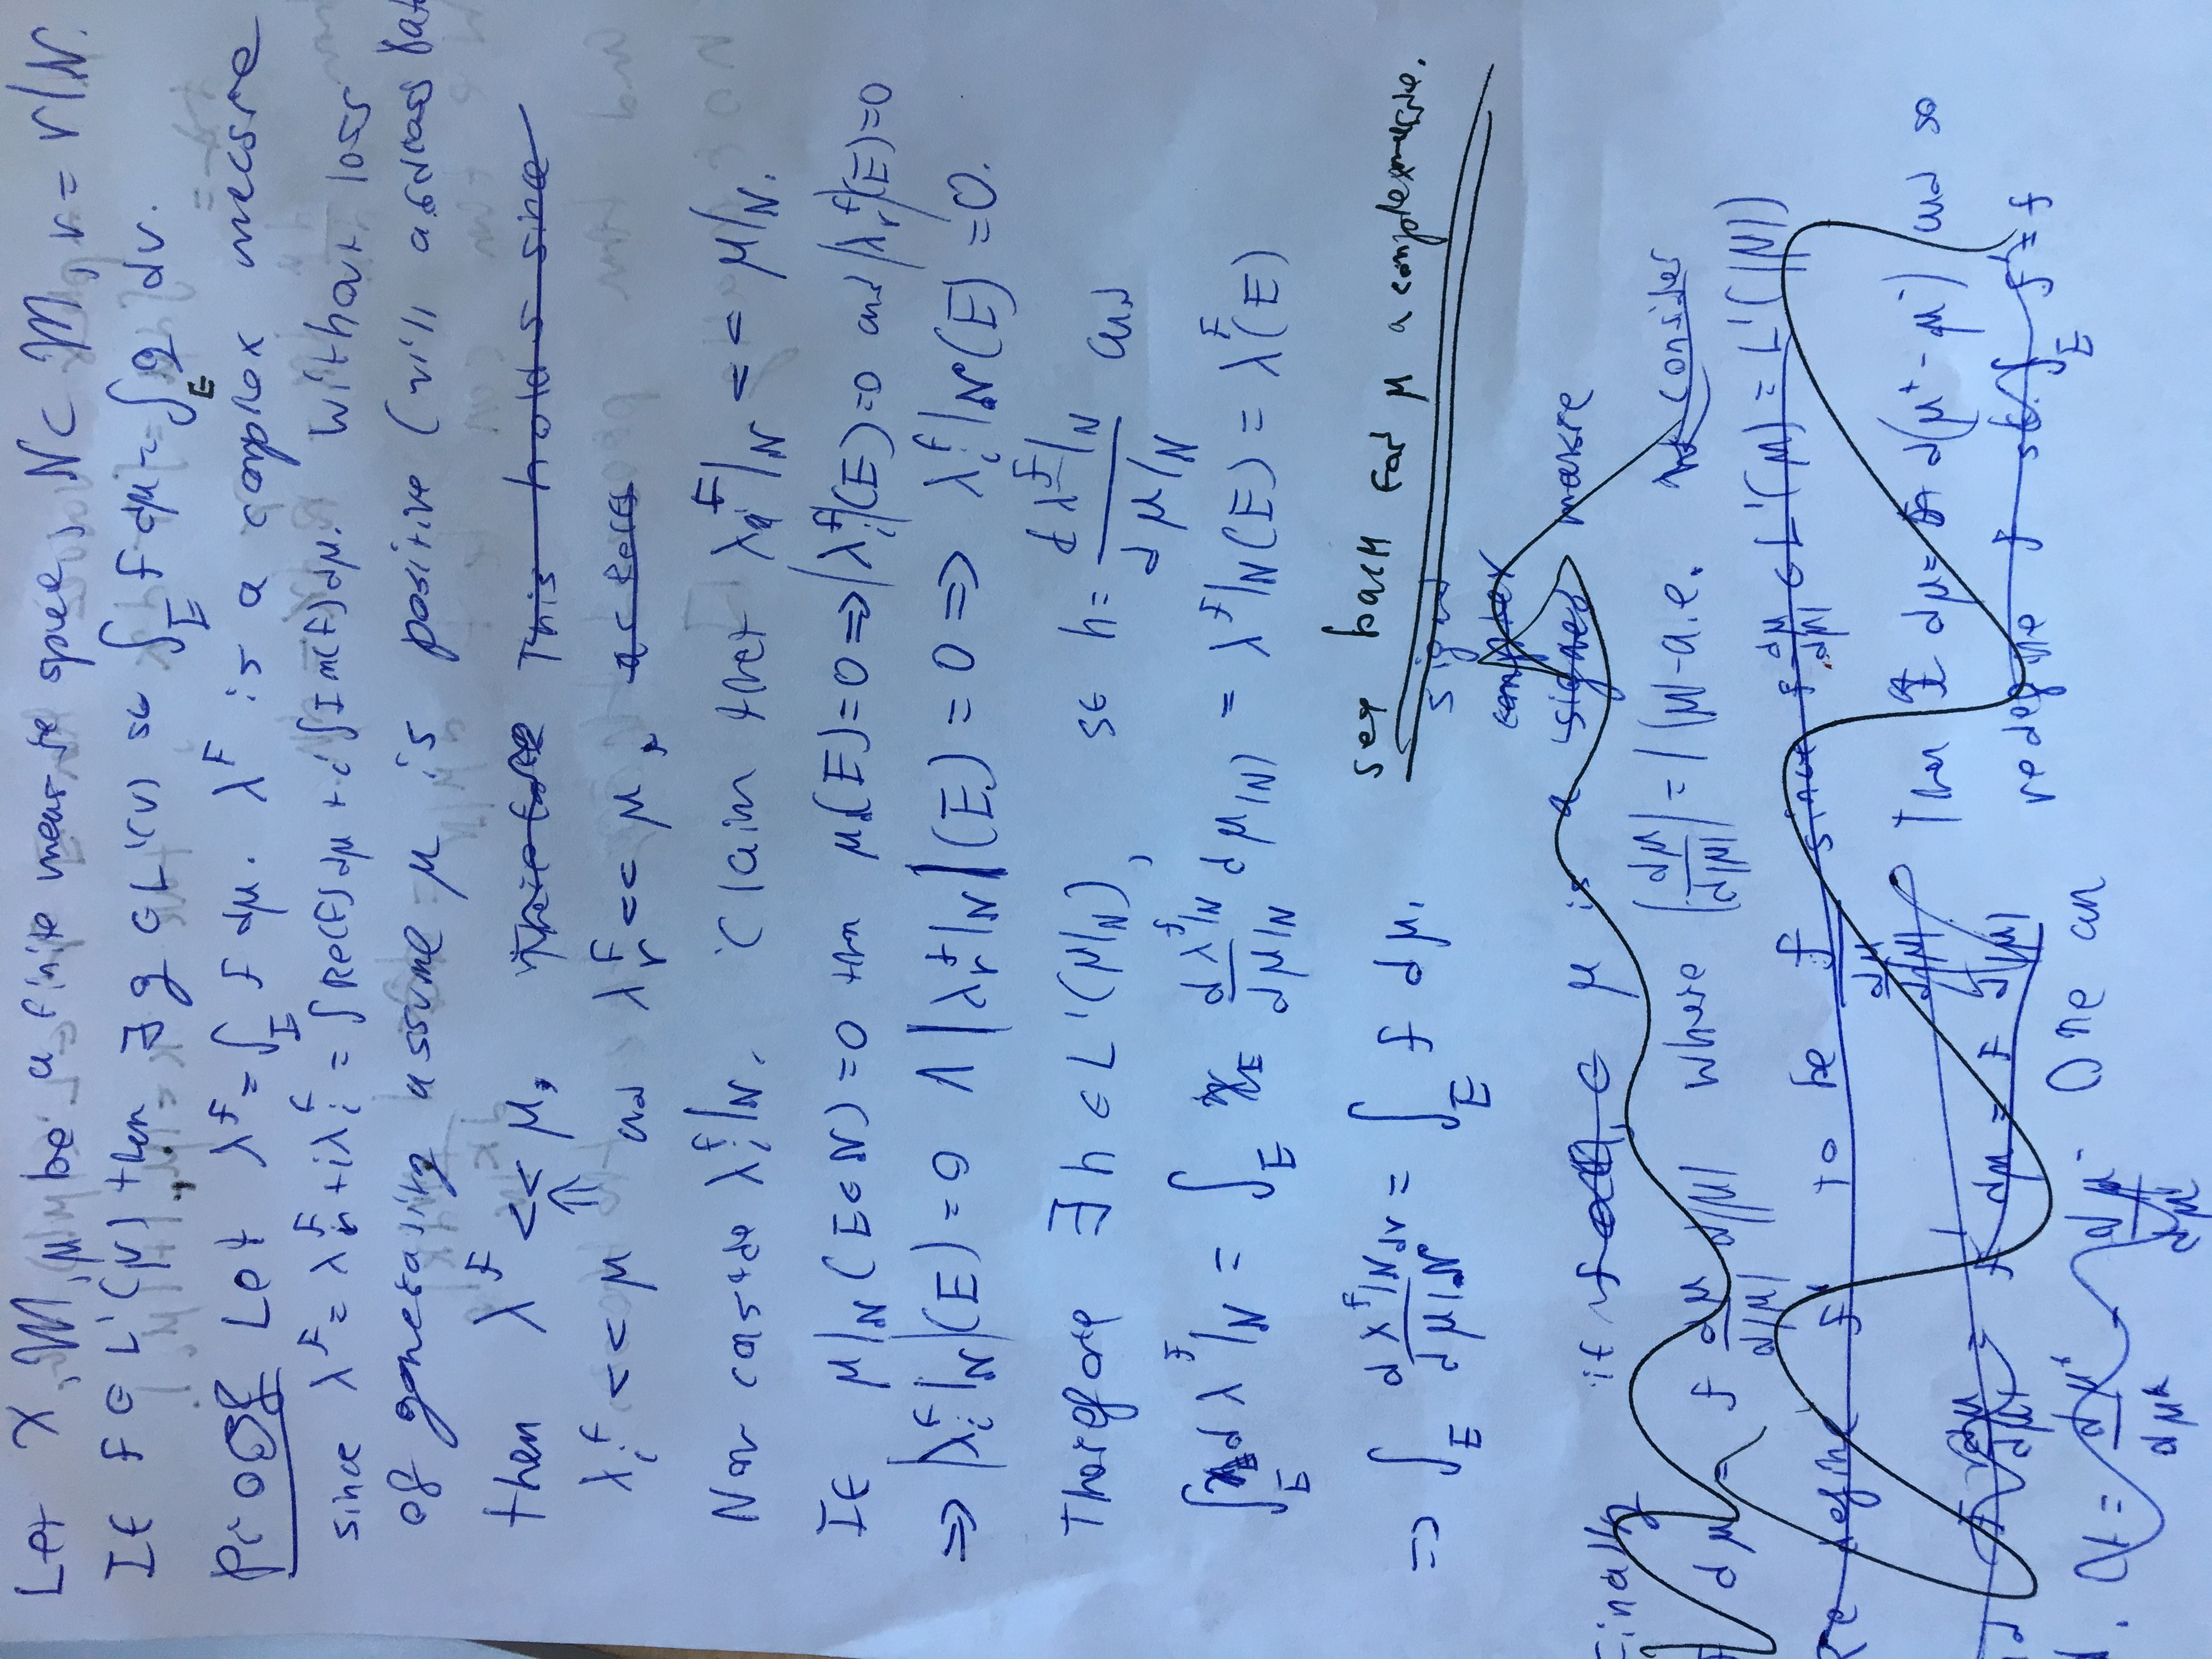
\includegraphics[angle=270,origin=c,width=1.3\linewidth]{File_001.jpeg}
    }
\end{figure}

\newpage
\begin{figure}[h]
    \vspace*{-2cm}
    \makebox[\linewidth]{
        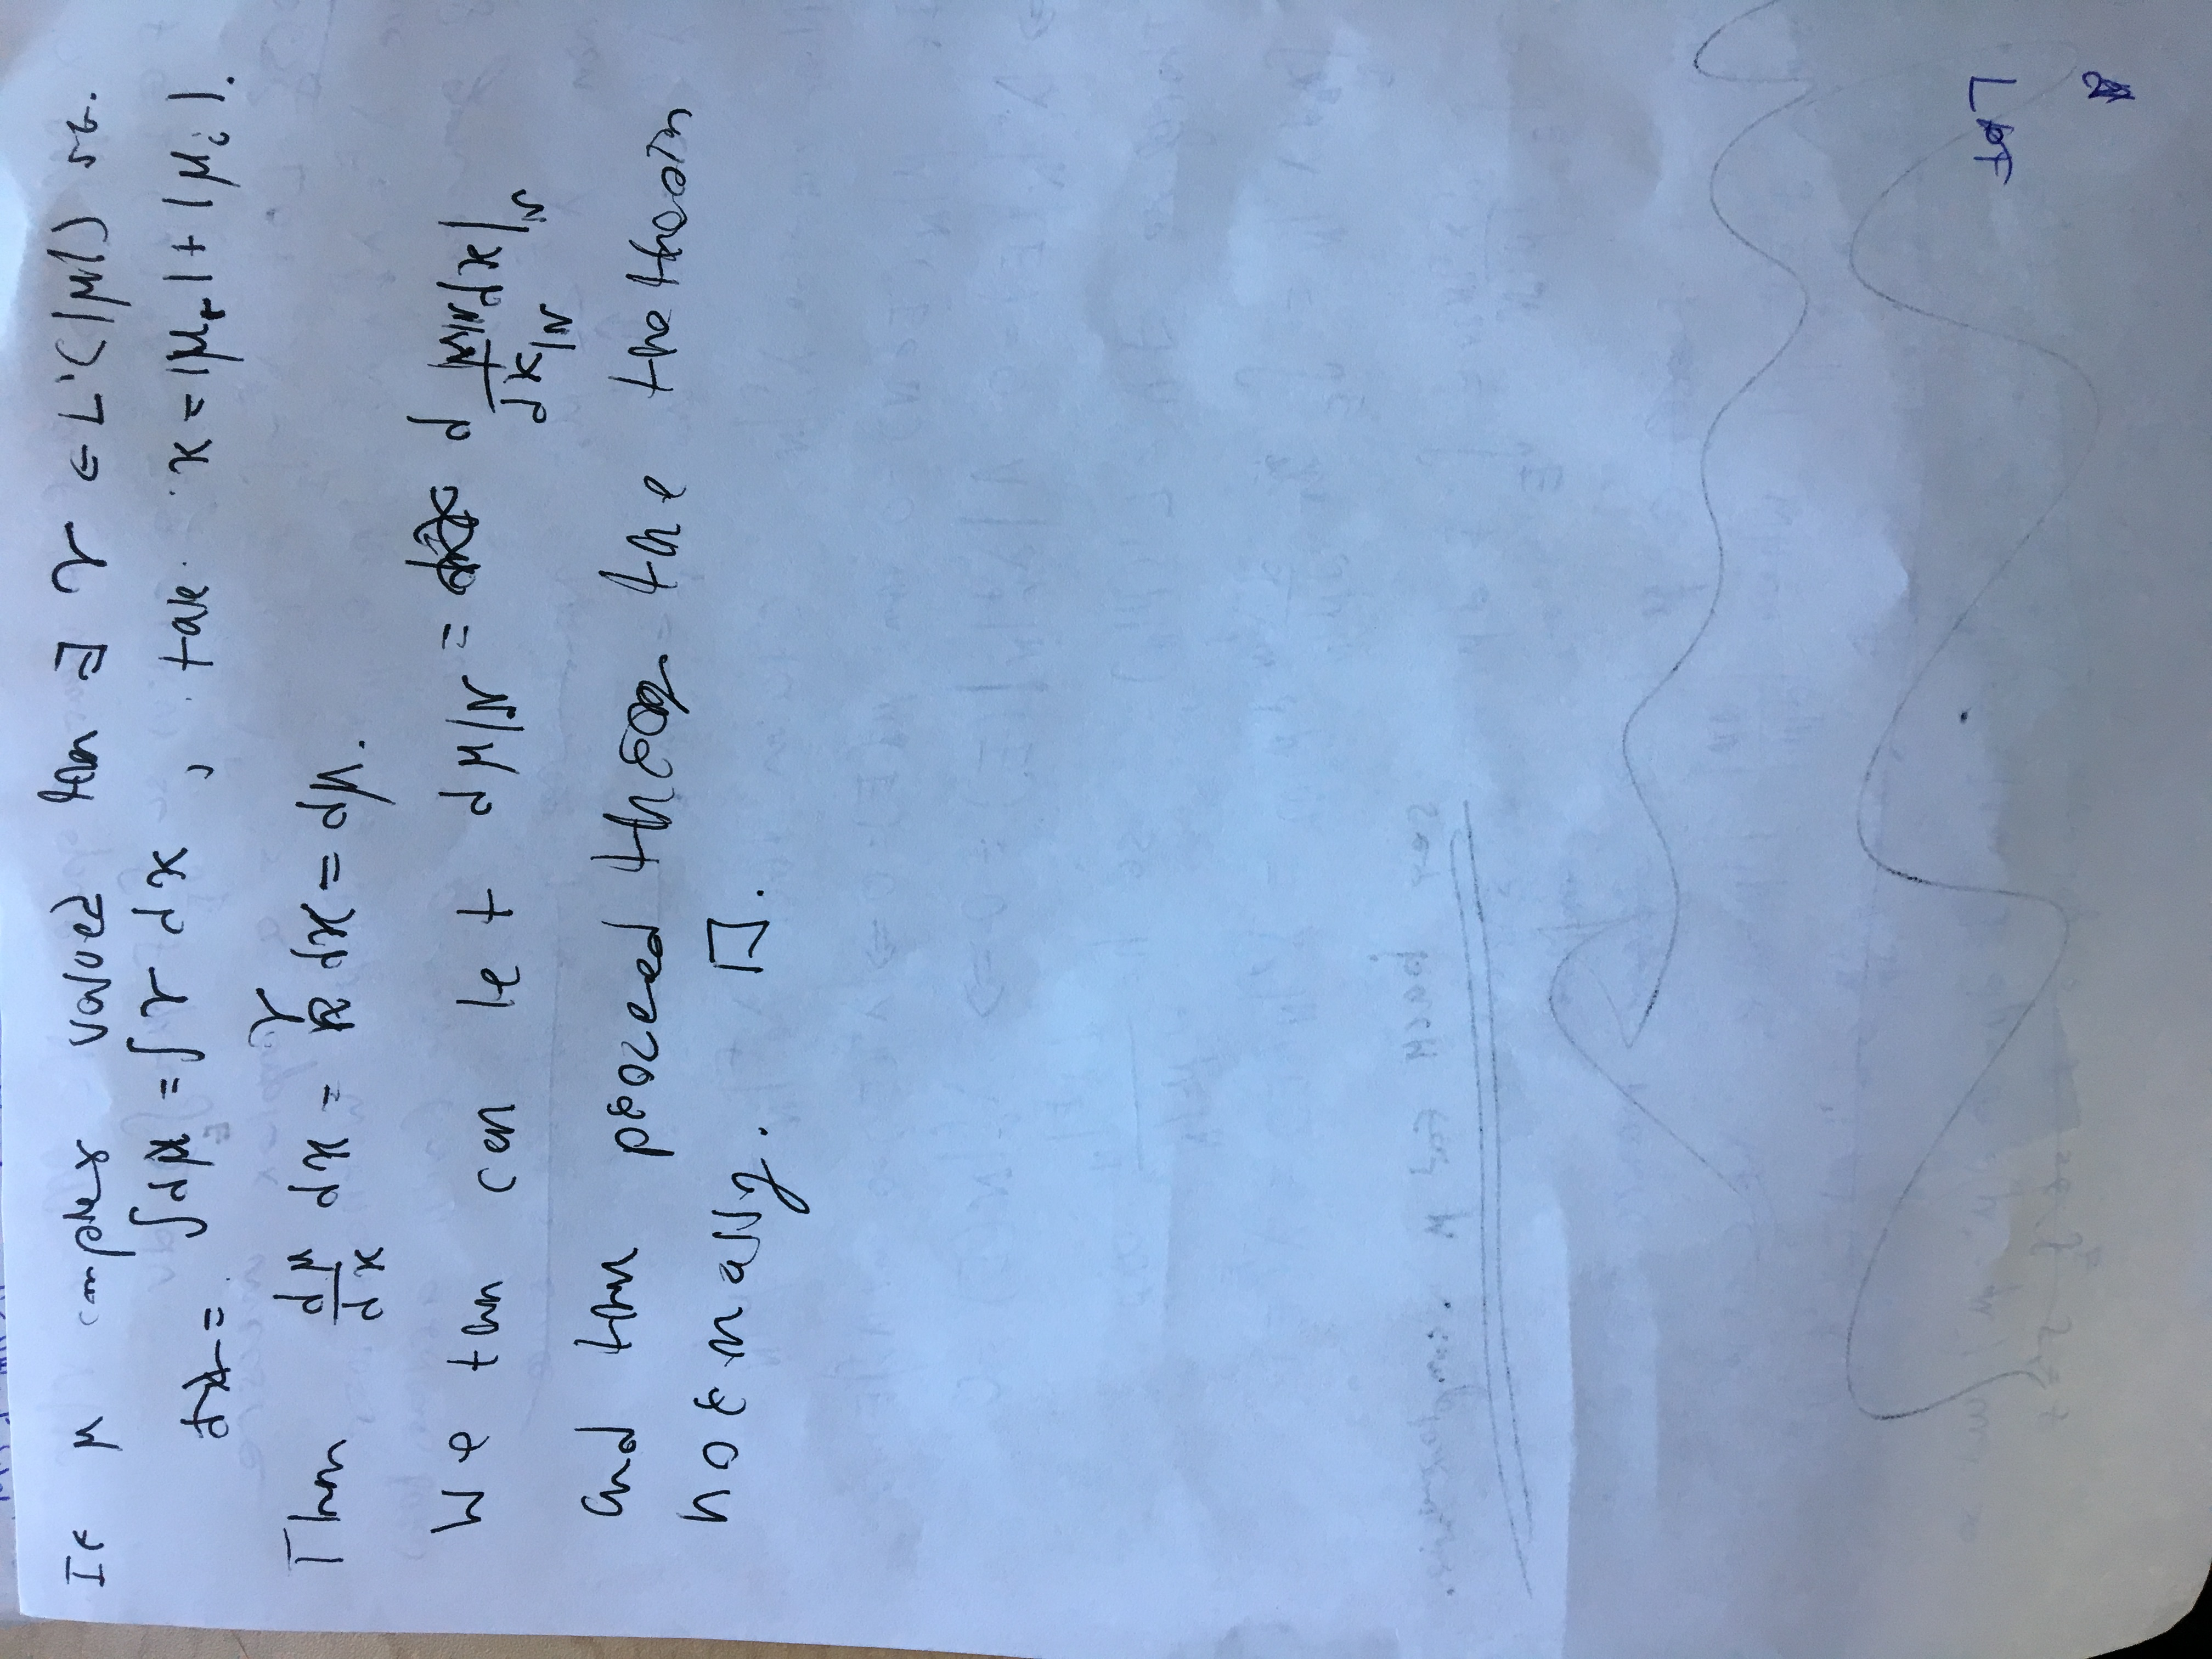
\includegraphics[angle=270,origin=c, width=1.3\linewidth]{File_000.jpeg}
    }
\end{figure}




\medskip \noindent {\bf (8.5)}\ 
(a)\ In problem (8.4), let $X=\integers$, let
$\scriptm=\scriptp(X)$.
Let $\scriptn\subset\scriptm$ be the collection of all
$E\subset\integers$ with this property: If $n$ is even
then $n\in E\Leftrightarrow n+1\in E$. 
Let $\mu$ be the natural counting measure on $\integers$.
Let $f,g$ be as above, where $f\in L^1(\integers,\scriptp(\integers))$
Give a concrete formula for $g$ in terms of $f$.\\


To first prove the statement we provide a definition.
\begin{definition}
	An $\scriptn$-chain, denoted $C_k^m$, is a set of contiguous integers
	such that
	\begin{equation*}
		C_k^m = \{2k, 2k+1, \dots, 2m, 2m+1\}
	\end{equation*}
	when $k\leq m$ and $k,m \in \mathbb{Z}.$
\end{definition}
We now give a lemma about $\scriptn$-chains.
\begin{lemma}
	If $E \in \scriptn$ then there is an $A \subset \mathbb{Z}^2$
	so that
	\begin{equation*}
		E = \bigcup_{(k,m) \in A} C_k^m.
	\end{equation*}
	This representation is not unique but can be reduced to a unique representation by
	merging adjacent $\scriptn$-chains until none can be merged.
\end{lemma}
\begin{proof}
	Given some $E \in \scriptn$ as defined above, consider all even $n \in E$. By defintion
	of $\scriptn$, $n+1 \in E.$ We claim that  if
	\begin{equation*}
		Q = \bigcup_{n \in E/2} C_{n/2}^{n/2}
	\end{equation*}
	then $E = Q$,
	where $E/2$ is the set of even members of $E$. Let $J = E \setminus Q$.
	If $n \in J$ then $n$ is such that $n \in E$, $n$ odd, and $n-1$ not in $E$. It follows in particular that $n-1$
	is not in $E$ since if it were then the $\scriptn$-chain $C_{(n-1)/2}^{(n-1)/2}$  would contain $n$ and $n-1$
	and therefore by $n-1 \in E$ even $C_{(n-1)/2}^{(n-1)/2}$ is a member of the union in $Q$. This would all contradict the fact that $n \in J$, so it must be that $n-1$ not in $E$. We claim that $J = \emptyset$. For all $ n \in J$, $n-1 \in \mathbb{Z}$ even implies $n \in E \iff n-1 \in E$ and since
	$n-1 \notin E$, $n \notin E$ unless $n = \emptyset.$ Therefore $J = \emptyset.$

	Now for every $E \in \scriptn$, $E$ is just a union of $\scriptn$ chains. A unique reduction exists but will not be proven.
\end{proof}
We now prove  (give) that there is a  concrete definition for $g$ in terms of $f.$
\begin{proof}
	Take $f \in L^1(\mu)$ then take $E \in \scriptn$. ow by the previous exercise there exists a $g\in L^{1}(\nu)$
	\begin{equation*}
		\int_E f d \mu = \sum_{y \in range(f)} \mu(f^{-1}(\{y\}))y = \sum_{y\in range(g)} \nu(g) (g^{-1}(\{y\})).
	\end{equation*}
	Since $g$ is $\scriptn$ measurable it must be that $g^{-1}(K) = \bigcup C_j^m$ for a measurable set $K$ by the previous lemma. There does not exist a $n \in g^{-1}(K)$ such that $g(n+1)\neq g(n)$ because is an $\scriptn$-chain $g^{-1}(\{g(n)\})$ containing $\{n, n+1\}$ and is a $\scriptn$-chain $g^{-1}(\{g(n+1)\})$ containing $\{n, n+1\}$ and so 
	\begin{equation*}
		g^{-1}(\{g(n)\}\cap \{g(n+1)\}) = g^{-1}(\{g(n)\})\cap g^{-1}(\{g(n+1)\})  \supset \{n, n+1\}.
	\end{equation*}
	and thus $\{g(n)\}$ must equal $\{g(n+1)\}$.

	With this in mind $g$ must take $1/2$ the value of $f(n)+f(n+1)$ on all even values in $E$ so as to equate the integral. This function is a measurable combination of constant functions on $\scriptn$-chains of cardinality $1$, so it is measurable. 
	Therefore if $E = \bigcup_{m\in A} C_{m/2}^{m/2}$
	\begin{equation*}
	\begin{aligned}
		 \int_E f d\mu = \sum_{y \in range(f)} \mu{(f^{-1}(y) \cap E)} y &= \sum_{y \in range(f)} \sum_{n \in f^{-1}(y)} \chi_E(n) \mu(\{n\}) {f(n)} \\
		&= \sum_{y \in range(f)} \sum_{n \in f^{-1}(y)/2} 2\frac{f(n)\chi_E(n) + f(n+1)\chi_E(n)}{2} \\
		&= \sum_{y \in range(g)} \sum_{n \in g^{-1}(y)/2} \nu(C_{n/2}^{n/2}) g(n) \chi_E(n) = \int_E g d\nu
	\end{aligned}
	\end{equation*}
	where $g(n) = g(n+1) = (f(n) + f(n+1))/2$, if $n$ is even and $ f^{-1}(x)/2$ is the even subset of the preimage of $x$. 
\end{proof}

(b)\ Now let $X=\integers^2$ and $\scriptm=\scriptp(X)$,
with $\mu$ equal to counting measure on $X$.
Let $\scriptn$ be the $\sigma$--algebra of subsets of $X$
of the form $B\times\integers$, where $B\subset\integers$
is arbitrary. Then $\mu|_\scriptn$ is not $\sigma$--finite.
Modify the conditional expectation construction by defining
$\nu(B\times\integers)$ to be the number of elements of $B$,
for any $B\subset\integers$. Show that for any $f\in L^1(\mu)$
there exists $g\in L^1(\nu)$ satisfying the required relation, 
and give a concrete formula for $g$ in terms of $f$.
\begin{proof}
	Because $f \in L^1(\mu)$ then $\int_X d\mu < \infty.$ Furthermore, $\int_{B\times\mathbb{Z}} f d\mu < \infty$.
	Thus define $m_b = \int_{\mathbb{Z}} f(b, z) d\mu(z) < \infty$. Now define $g(b,x) = m_b$ for all $x$.
	Then if $E \in \scriptn$ and $I(b) = \int_{\mathbb{Z}} f(b,z) d\mu(z) = m_b$, by the FubiniTonelli theorem
	\begin{equation*}
	\begin{aligned}
		\infty > \int_E f d\mu = \sum_{y \in range(f)} y \mu(f^{-1}(y) \cap E) &= \sum_{m_b \in range(I)}  m_b \mu_1(I^{-1}(m_b) \cap B) \\
		(\text{by finiteness of the sum})\;\;&= \sum_{m_b \in range(I)}m_b \sum_{b \in I^{-1}(m_B) \cap B}   \nu(\{b\} \times \mathbb{Z}) \\
		&= \sum_{m_b \in range(g(\cdot, x))}m_b \sum_{b \in g(x,\cdot)^{-1}(m_b) \cap B}   \nu(\{b\} \times \mathbb{Z}) \\
		&= \sum_{m_b \in range(g(\cdot, x))} m_b  \nu(g(\cdot, x))^{-1}(m_b) \cap B \times \mathbb{Z})  \\
		(\text{by }g(b,x) = m_b\text{ for all }x)\;\; &= \sum_{m_b \in range(g)} m_b  \nu(g^{-1}(m_b) \cap (B \times \mathbb{Z}))  \\
	\end{aligned}
	\end{equation*}
	where $\mu_1$ is the first projection measure (which is nameley equal to $\nu$).
\end{proof}

\medskip \noindent {\bf (8.6)}\ (Folland problem 3.18)\ 
Prove Proposition~3.13(c) of our text:
For any complex measure $\nu$ on a measurable space $(X,\scriptm)$,
$L^1(\nu)=L^1(|\nu|)$, and for any $f\in L^1(\nu)$,
$|\int f\,d\nu| \le \int |f|\,d|\nu|$.
\begin{proof}
	First let $\mu = |\nu_r| + |\nu_i|$ and then by the book
	$d\nu = g d\mu$ with $g \in L^1(\mu)$ and $d|\nu| = |g| d\mu$ with $g \in L^1(\mu).$
	Finally by Prop 3.13 (a,b), $d\nu = h d|\nu|$ where $h \in L^1(|\nu|)$ and $|h| = 1$ $|\nu|$-a.e.
	Next $f d\nu = fg d\mu$ and $f,g \in L^1(\mu)$ by a proposition of the chapter.
	And we therefore have
	\begin{equation*}
	  	\begin{aligned}
		f d\nu &= fg d\mu   	 \\
		&= f\frac{d \nu}{d |\nu|} d|\nu|&\;\;\;\ f \frac{d \nu}{d |\nu|} \in L^1(|\nu|) \\
		&=  f\frac{d \nu}{d |\nu|}  |g| d\mu &\;\;\;\ f\frac{d \nu}{d |\nu|}  |g|\in L^1(\mu) \\
	  	\end{aligned}
	  \end{equation*}  
	  Then since $|\frac{d \nu}{d |\nu|}|  = |h| =1$ $|\nu|$-a.e we get (using the first and last equation from above)
	  \begin{equation*}
	  \begin{aligned}
		|f| d\nu &= |fg| d\mu    &= |fg| d\mu	 \\
		&= |f \frac{d\nu}{d\mu}| d\mu &= |f \frac{d |\nu|}{d \mu}|d\mu \\
		&= |f| d\nu &= |f| d|\nu|
	  	\end{aligned}
	  \end{equation*}
	  Now the equality gives $\int f d\nu < \infty$  if and only if $\int f d|\nu| < \infty$. So $f \in L^1(|\nu|)$
	  if and only if $f \in L^1(\nu)$ and so the function spaces are equal.

	  Finally \begin{equation*}
	  	\begin{aligned}
	  		\left|\int f\ d\nu\right| &\leq \int |f|\ d\nu  = \int |f|\frac{d \nu}{d |\nu|} d|\nu| \\
	  		&\leq \int \left|f\frac{d \nu}{d |\nu|}\right| d|\nu| = \int |f| d|\nu| \\
	  	\end{aligned}
	  \end{equation*}
	  by $|\frac{d \nu}{d |\nu|}| =1$ a.e.
\end{proof}

\medskip \noindent {\bf (8.7)}\ (Folland problem 3.19)\ 
Let $\nu,\mu$ be complex measures, and let $\lambda$ be a positive measure,
on a common measurable space.
Show that $\nu\perp\mu$ if and only if $|\nu|\perp |\mu|$.
Show that $\nu\ll \lambda $ if and only if $|\nu|\ll|\lambda$.
\begin{proof}
	If $\nu \perp \mu$ then there exist $A,B$ such that $A \bigcup B = X$
	and $|\nu_i|(A) + |\nu_r|(A) = 0$ and $|\mu_r|(B) + |\mu_i|(B) = 0$.
	Let $f, g$ such that $d\nu = f d(|\nu_i|(A) + |\nu_r|)$ and
	$d \mu = g d(|\mu_r| + |\mu_i|)$. 
	Without loss of generality we will treat $\nu$ and then assume the same treatment for $\mu$
	on $B$
	It follows that
	\begin{equation*}
		|\nu|(A) = \int_A |f| d(|\nu_i|(A) + |\nu_r|) = 0
	\end{equation*}
	because $(|\nu_i|(A) + |\nu_r|)(A) = 0$.
	Thus $|\nu| \perp |\mu|.$

	In the other direction If $|\nu|(A) =0$ and $|\mu|(B) = 0$ then $\nu \ll |\nu|$ implies
	that $A$ is a $\nu$-nullset. Likewise
	$\mu \ll |\mu|$ implies that $B$ is a $\mu$-nullset.

	Now if $\nu \ll \lambda$ then $E \lambda$ null implies that $E$ $\nu$ null.
	Again 
	\begin{equation*}
		|\nu|(A) = \int_A |f| d(|\nu_i|(A) + |\nu_r|) = 0
	\end{equation*}
	by $d(|\nu_i|(A) + |\nu_r|) = 0$. 

	In the other directon if $|\nu| \ll \lambda$ then if $E \lambda$ null
	then $E$ is $|\nu|$ null. Since $\nu \ll |\nu|$ then $E$ is $\nu$ null.
	Therefore $\nu \ll \lambda$

\end{proof}

\medskip \noindent {\bf (8.8)}\ (Folland problem 3.21)\ 
Let $\nu$ be a complex measure on $(X,\scriptm)$.
For any $E\in\scriptm$ define measures $\mu_j$, for $j\in\{1,2,3\}$,
as in the problem statement in our text. 
Show that these measures are equal to one another,
and are all equal to $|\nu|$. 
\begin{proof}
	Let $\mu_j(E)$ be given from the text and the sets over whuich they are the resultant supremums be $S_j(E)$. 

	\textbf{First}. We will show that $\mu_3 \leq \mu_1$. Since $\mu_3$ is the supremum there exists a sequence of $L^1(\nu)$ measurable functions $f_n$ with $|f_n| \leq 1$ so that $a_n=|\int_E f_n d\nu| \to \mu_3(E)$. If we show that a sequence in $S_1(E)$ tends to $\mu_1(E)$ above $a_n$ then $\mu_3 \leq \mu_1$. For each $n$ there is a sequence of simple functions $phi_{n,m}$ approximating $f_n$ so that $\int|\phi_{n,m} - f_n| d\nu \to 0$ as $m \to \infty$.
	Then consider the embodiment of $\phi_{n,n}$ in $S_3$; that is
	\begin{equation*}
		\begin{aligned}
			\left|\left|\int_E \phi_{n,n} d\nu \right| - \mu_3(E)\right| &= \left|\left|\int_E \phi_{n,n} d\nu \right| - \left|\int_E f_n d\nu \right| - \mu_3(E) + \left|\int_E f_n d\nu \right|\right| \\
			&\leq \left|\left|\int_E \phi_{n,n} d\nu \right| - \left|\int_E f_n d\nu \right|\right| + \left| \left|\int_E f_n d\nu \right|  - \mu_3(E)\right| \\
			&< \left|\left|\int_E \phi_{n,n} d\nu \right| - \left|\int_E f_n d\nu \right|\right| + \epsilon/2 \\
			&\leq \int_E \left|\left|\phi_{n,n} \right| - \left| f_n \right|\right| d\nu  + \epsilon/2 \\
			&\leq \int_E \left|\phi_{n,n}  - f_n \right| d\nu  + \epsilon/2  < \epsilon\\
		\end{aligned}
	\end{equation*}
	Knowing that there is a sequence of simple function $\psi_n = \phi_{n,n}$ whose embodiment in $S_3$ tends towards the supremum with $|\psi_n| \leq 1$ and $|\psi_E \psi_n| \to \mu_3(E).$
	Next we expand the definition of a simple function using the standard representation on $E$ and get
	\begin{equation*}
		\begin{aligned}
			\left|\int_E \psi_n d \nu\right| \leq \int_E |\psi_n| d \nu = \sum_{j=1}^m |y_n^j| \nu(E_j)
			\leq \sum_{j=1}^m |y_n^j| |\nu(E_j)| \in S_1(E)^\mathbb{N}
		\end{aligned}
	\end{equation*}
	where $ S_1(E)^\mathbb{N}$ denotes the set of sequences in $S_1(E)$. Since the embodiment of $\psi_n$ in $S_3(E)$ tends
	towards the supremum and is dominated by a sequence in $S_1(E)$ we have that the supremum of $S_(E)1$ dominates $S_3(E)$ and $\mu_3(E) \leq \mu)1(E).$

	\textbf{Second}. We would like to show $\mu_1 \leq \mu_2$.  We will use the same technique as before. Let $(a_n) \in S_1(E)^\mathbb{N}$ so that $a_n \to \mu_1(E).$ Then 
	\begin{equation*}
		a_n = \sum_{j=1}^{m_n} \left|\nu (E_j^n)\right|\;\;\;\;\bigsqcup_{j=1}^m E_j^n = E.
	\end{equation*}
	Let $b_n = \sum_{j=1}^{\infty} \left|\nu (K_j^n)\right|\;\;\;\;\bigsqcup_{j=1}^m K_j^n = E$ where $K_j^n = \emptyset$ when
	$j > m_n$ and $K_j^n = E_j^n$ otherwise. Therefore $K_p^n \cap K_q^n = \emptyset$ where $p,q \geq m_n, q > p$ so by disjointness of the $E_j^n$ then $K_j^n$ are disjoint. Now $a_n \leq b_n$ for all $n$ and since $a_n \to m_1(E)$ we use the same domination argument as before. Therefore $\mu_1(E) \leq \mu_2(E).$

	\textbf{Third.} We would like to show that $\mu_2 \leq |\nu|.$ This is immediate from one of the corrolaries (3.13). Consider $(a_n) \in S_2(E)^\mathbb{N}$ such that $a_N \to \mu_2$. Then
	\begin{equation*}
	\begin{aligned}
		a_n &= \sum_{j=1}^{\infty} \left|\nu (E_j^n)\right|\;\;\;\;\;\;\;\;&\bigsqcup_{j=1}^\infty E_j^n = E. \\
			&\leq \sum_{j=1}^{\infty} \left|\nu\right| (E_j^n) \\
			&= |\nu|(E) &\text{(by disjointness)}
	\end{aligned}
	\end{equation*}

	\textbf{Fourth.} We lastly would like to show that $\mu_3 = |\nu|$. We will use the Radon-Nikodym theorem.
	Let $f = \frac{d\nu}{d|\nu|}$, this exists by $\nu \ll |\nu|$. Then $\left|\int_E f d\nu \right| \leq \int_E |f| d|\nu|.$ But $\int_E |f| d|\nu|$ is just $\int_E d|\nu|$ because $|f| = |\frac{d\nu}{d|\nu|}|$ is $1$ $|\nu|$-a.e. Finally by
	$L^1(|\nu|) = L^1(\nu)$ and $1 = |f| \leq 1$, $|\nu|$-a.e. we have that $|f| \in S_3(E).$ Now suppose that there were a $g \in S_3(E)$ so that $g > |f|$ then $|g| > 1$ $|\nu|$-a.e. and this is not possible. Therefore $|f|$ is the supremum.


	\textbf{Conclusion}. We've shown for aribtraty $E$ $|\nu|=\mu_3 \leq \mu_1 \leq \mu_2\leq|\nu|$ and so $\mu_1 = \mu_2 = \mu_3 = |\nu|.$ This completes the proof.


\end{proof}
\end{document}\end
